\documentclass[10pt]{article}

\usepackage[T1]{fontenc}
\usepackage{lmodern}
\usepackage{microtype}
\usepackage[margin=0.82in]{geometry}
\usepackage{amsmath,amssymb}
\usepackage{booktabs}
\usepackage{tabularx}
\usepackage{array}
\usepackage{multirow}
\usepackage{enumitem}
\usepackage{xcolor}
\usepackage{graphicx}
\usepackage{caption}
\captionsetup{hypcap=false}
\usepackage{tikz}
\usetikzlibrary{arrows.meta,positioning,fit,calc}
\usepackage{pgfplots}
\pgfplotsset{compat=1.18}
\usepackage[numbers,sort&compress]{natbib}
\usepackage[hidelinks]{hyperref}
\usepackage[nameinlink,noabbrev]{cleveref}

\definecolor{safeblue}{HTML}{276FBF}
\definecolor{safegreen}{HTML}{2A9D8F}
\definecolor{safecoral}{HTML}{E76F51}
\definecolor{safegold}{HTML}{D89B27}
\definecolor{safelight}{HTML}{F2F5F7}
\definecolor{safedark}{HTML}{23313F}

\hypersetup{
  pdftitle={SafeDesk: Evidence-Grounded Runtime Governance for Long-Horizon Tool-Using Agents},
  pdfauthor={Authors withheld in working draft},
  pdfsubject={Runtime governance for tool-using language-model agents},
  pdfkeywords={LLM agents, tool calling, runtime governance, verification, recovery, context management},
  colorlinks=true,
  linkcolor=safeblue,
  citecolor=safeblue,
  urlcolor=safeblue
}

\newcolumntype{Y}{>{\raggedright\arraybackslash}X}
\newcolumntype{R}{>{\raggedleft\arraybackslash}X}
\newcommand{\safedesk}{\textsc{SafeDesk}}
\newcommand{\pending}{\textsc{Pending}}
\newcommand{\measured}{\textsc{Measured}}
\newcommand{\diagnostic}{\textsc{Diagnostic}}
\newcommand{\tgc}{\mathrm{TGC}}
\newcommand{\sgc}{\mathrm{SGC}}
\setlength{\emergencystretch}{1.5em}

\title{\safedesk: Evidence-Grounded Runtime Governance\\
for Long-Horizon Tool-Using Agents}
\author{Authors withheld in this working draft\\
\small Affiliation and contact information to be inserted before public submission}
\date{July 22, 2026}

\begin{document}
\maketitle

\begin{abstract}
Language-model agents can operate applications, databases, and external services
through function calls, yet failures in long-horizon tasks extend beyond isolated
reasoning errors. Agents may drift from the original goal, omit subgoals, invoke
invalid or unavailable tools, repeat side-effecting actions, retry blindly, or
declare completion without evidence from the environment. We present \safedesk,
an evidence-grounded runtime governance framework that does not update model
weights. It represents execution as task-constrained state transitions and
coordinates four modules: State \& Verification, Tool Execution Guard, Recovery
Controller, and Context Manager. Structured traces record state, evidence,
effects, interventions, and recovery decisions for diagnosis and ablation.

As a diagnostic baseline, a repaired no-thinking DeepSeek V4 Flash
function-calling runner achieves 41.73\% Task Goal Completion (TGC) and 29.50\%
Scenario Goal Completion (SGC) on all 417 AppWorld \texttt{test\_challenge}
tasks. Failed tasks consume 737,614 tokens on average, compared with 130,653 for
successful tasks. Max-turn exhaustion, out-of-schema attempts, and duplicate
calls are strongly associated with failure. We also report a 278-task
$\tau^2$-bench diagnostic baseline, an implementation inventory, a reproducible
data protocol, and a preregistered matched-model evaluation design. Full
\safedesk{} outcome experiments are pending; consequently, this draft makes no
claim that \safedesk{} improves benchmark performance.
\end{abstract}

\noindent\fcolorbox{safegold}{safelight}{%
\parbox{0.95\linewidth}{\small\textbf{Evidence status.}
System implementation, baseline measurements, and the evaluation protocol are
complete. Matched Qwen3-14B baseline, \safedesk{} intervention, and ablation
experiments have not yet been run. Empty result cells are deliberately marked
\pending{} rather than filled with estimates.}}

\section{Introduction}

ReAct-style agents interleave reasoning and environmental action, enabling
language models to use APIs, databases, and search systems
\citep{yao2023react}. As tasks expand from a single lookup to cross-application,
multi-step workflows with side effects, longer prompts and larger turn budgets do
not by themselves guarantee reliability. Errors accumulate across layers: the
active goal drifts during conversation; a tool selector omits a required API;
writes are scheduled against stale state; a tool reports success without the
expected environmental change; a failed step is repeated; and the final response
contradicts the actual state.

AppWorld provides nine applications, 457 APIs, and 750 tasks evaluated through
state-based tests and collateral-damage checks \citep{trivedi2024appworld}.
$\tau$-bench places tool use inside dynamic user conversations governed by domain
policies and evaluates the final database state and repeated-trial reliability
\citep{yao2024taubench}. Together, these benchmarks expose a gap between
generating plausible actions and governing a reliable execution lifecycle.

We ask whether a model-agnostic runtime can improve controllability,
interpretability, and resource efficiency without updating model weights. Recent
agentic reinforcement learning (RL) methods substantially improve Qwen3-14B on
multi-turn tool tasks \citep{hu2026seeupo}; the AppWorld leaderboard also records
a high-scoring Qwen3-14B AgentRL entry \citep{appworldleaderboard2026}. Rather than
replace training, \safedesk{} explores a complementary layer: explicit task
contracts, evidence, effect tracking, guarded execution, typed recovery, and
bounded context construction.

Our contributions are:
\begin{enumerate}[leftmargin=*,itemsep=2pt]
  \item a unified runtime model over task state, evidence, effects, failures,
        context, and trace events;
  \item four composable governance modules that convert completion from a model
        assertion into an evidence-backed decision;
  \item a framework-independent implementation with versioned JSON Schemas,
        tracing, DeerFlow integration \citep{deerflow2026}, and AppWorld adapters;
  \item a reproducible measurement protocol spanning goal completion, false
        completion candidates, invalid and duplicate calls, recovery, tokens,
        latency, and infrastructure failures; and
  \item a complete diagnostic baseline and a frozen evaluation matrix that
        separates measured evidence from untested claims.
\end{enumerate}

\section{Problem Formulation}

\subsection{Long-horizon tool tasks}

We represent a task contract as
\begin{equation}
  \mathcal{T} = (G, C, P, V),
\end{equation}
where $G$ is the set of goals and subgoals, $C$ contains user constraints and
invariants, $P$ is the tool and business policy, and $V$ specifies the evidence
required for completion. At step $t$, the agent observes a context view $X_t$ and
proposes one or more actions $A_t$. Tool execution produces observations $O_t$
and an environmental state change $\Delta S_t$.

Unlike a message-only harness, \safedesk{} maintains six distinct objects:
\begin{itemize}[leftmargin=*,itemsep=1pt]
  \item \textbf{Task State $S_t$:} goals, constraints, known entities, blockers,
        and execution phase;
  \item \textbf{Evidence Board $E_t$:} sourced, timestamped, and scoped facts;
  \item \textbf{Effect Ledger $L_t$:} intended and observed writes, idempotency
        keys, and verification state;
  \item \textbf{Failure State $F_t$:} failure type, recoverability, attempts, and
        remaining budget;
  \item \textbf{Context Pack $C_t$:} a bounded model-facing projection rather
        than the full raw trajectory; and
  \item \textbf{Trace $R$:} an auditable record of calls, decisions, state
        transitions, verification, and recovery.
\end{itemize}

\subsection{Evidence-grounded completion}

A call to \texttt{complete\_task} expresses intent; it is not proof of success.
The completion gate is modeled as
\begin{align}
\operatorname{Complete}(S_t,E_t,L_t) =
  &\bigwedge_{g \in G_{\mathrm{req}}} \operatorname{satisfied}(g) \nonumber\\
  &\land \bigwedge_{e \in L_{\mathrm{req}}} \operatorname{verified}(e) \nonumber\\
  &\land \neg\operatorname{unresolvedBlocker}(S_t)
   \land \operatorname{policySatisfied}(P).
\end{align}
The gate permits termination only when required subgoals, write effects, blockers,
and policy conditions are resolved by admissible evidence.

\subsection{Research hypotheses}

We preregister four hypotheses. \textbf{H1} predicts higher TGC and SGC under a
matched \safedesk{} runtime. \textbf{H2} predicts lower false-completion,
invalid-call, duplicate-write, and max-turn rates. \textbf{H3} predicts lower
failed-task token tails after accounting for verification overhead. \textbf{H4}
predicts distinguishable contributions from all four modules. These are pending
hypotheses, not findings in the current draft.

\section{Related Work}

ReAct interleaves reasoning and action \citep{yao2023react}, while Reflexion uses
linguistic feedback and episodic memory to improve later attempts
\citep{shinn2023reflexion}. These methods alter reasoning or feedback; \safedesk{}
provides an external control plane that can still reject, schedule, verify, or
recover an action generated by any compatible model.

ToolEmu emulates tools to identify risky agent behavior and evaluates safety
failures \citep{ruan2024toolemu}. GuardAgent uses a separate guard agent and
executable rules to moderate target-agent actions \citep{xiang2025guardagent}.
\safedesk{} extends the protected surface from individual safety decisions to the
full execution lifecycle, including goal state, effects, post-action verification,
recovery, completion, and context budgets.

Qwen3 exposes both thinking and non-thinking inference modes
\citep{yang2025qwen3}. Agentic RL methods such as SeeUPO show that training can
improve multi-turn policies \citep{hu2026seeupo}. Runtime governance and training
are complementary: training changes the proposal distribution, whereas runtime
controls provide deterministic constraints, auditability, and cross-model reuse.

\section{System Design}

\begin{figure*}[t]
\centering
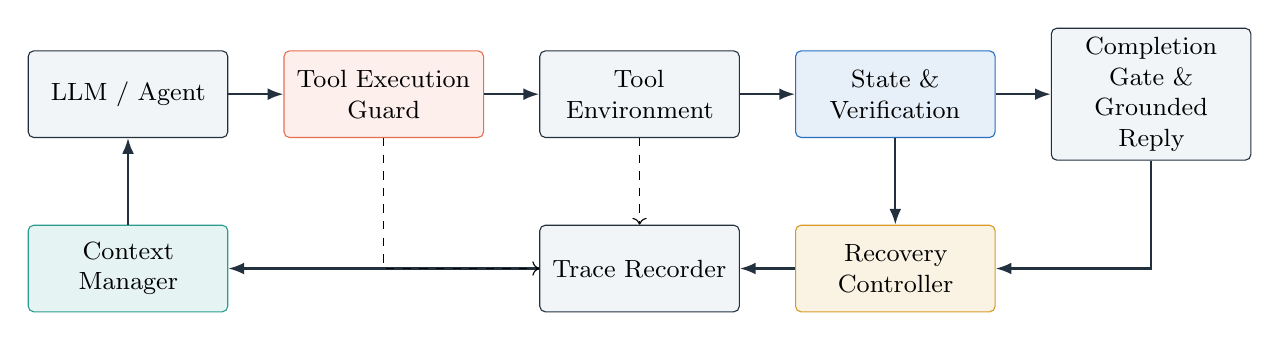
\begin{tikzpicture}[
  node distance=11mm and 7mm,
  box/.style={draw=safedark, rounded corners=2pt, fill=safelight,
              minimum height=11mm, align=center, font=\small,
              text width=23mm},
  core/.style={box, fill=safeblue!11, draw=safeblue},
  guard/.style={box, fill=safecoral!11, draw=safecoral},
  recovery/.style={box, fill=safegold!13, draw=safegold},
  context/.style={box, fill=safegreen!12, draw=safegreen},
  arr/.style={-{Latex[length=2mm]}, thick, draw=safedark}
]
\node[box] (llm) {LLM / Agent};
\node[guard, right=of llm] (guard) {Tool Execution\\Guard};
\node[box, right=of guard] (env) {Tool\\Environment};
\node[core, right=of env] (verify) {State \&\\Verification};
\node[box, right=of verify] (finish) {Completion Gate \&\\Grounded Reply};
\node[context, below=of llm] (context) {Context\\Manager};
\node[box, below=of env] (trace) {Trace Recorder};
\node[recovery, below=of verify] (recover) {Recovery\\Controller};

\draw[arr] (llm) -- (guard);
\draw[arr] (guard) -- (env);
\draw[arr] (env) -- (verify);
\draw[arr] (verify) -- (finish);
\draw[arr] (verify) -- (recover);
\draw[arr] (finish) |- (recover);
\draw[arr] (recover) -- (trace);
\draw[arr] (trace) -- (context);
\draw[arr] (context) -- (llm);
\draw[dashed,->] (env) -- (trace);
\draw[dashed,->] (guard) |- (trace);
\end{tikzpicture}
\caption{The \safedesk{} runtime loop. The model proposes actions; guarded
execution, environmental evidence, and completion are separate decisions. Dashed
arrows denote structured trace emission.}
\label{fig:architecture}
\end{figure*}

The coordinator processes each turn as follows: reduce task state; construct the
context pack; normalize actions; validate schema and policy; schedule dependencies;
preflight effects; execute tools; project results; update evidence; verify writes;
assess progress; classify failures; select recovery; and evaluate completion.
Versioned contracts connect stages without depending on a framework-specific
message object.

\subsection{State \& Verification}

Task State converts the request into tracked subgoals, constraints, entities, and
blockers. Evidence Board stores facts with source, time, freshness, and subgoal
scope. Effect Ledger records write intent, target resource, idempotency key,
execution status, and verification status. Post-action Verification performs
readback or state-difference checks. Completion Gate aggregates subgoal, evidence,
effect, policy, and blocker conditions. Response Grounding prevents a final answer
from claiming success when the verified state disagrees.

\subsection{Tool Execution Guard}

The guard normalizes model calls into an Action IR and validates tool names,
required fields, types, and enumerations. Policy checks enforce authentication,
confirmation, permission, and domain rules. Effect preflight detects duplicate or
high-risk writes using the ledger and idempotency keys. The dependency scheduler
can execute independent reads serially while preserving all tool-call results; a
state-changing batch executes only the first currently safe write and explicitly
marks deferred calls as unexecuted. Dynamic Tool Resolver can expand the active
schema from the catalog when evidence shows that a required API is missing.

\subsection{Recovery Controller}

Failures are classified into parameter, schema, entity, permission, policy, tool,
environment, state-mismatch, context, or unknown categories. Typed Recovery maps
categories to parameter repair, re-query, tool resolution, state refresh, local
replanning, or bounded retry. Progress Monitor compares adjacent states, evidence,
and effects. Stagnation Detector combines repeated signatures, semantically
redundant reads, repeated failure types, and consecutive no-progress turns.
Recovery Budget bounds attempts by failure class and total cost.

\subsection{Context Manager}

Context Manager builds a bounded model-facing projection. It preserves the task,
hard constraints, unsatisfied goals, verified facts, unresolved failures, and
idempotency keys; projects large tool results to necessary fields; summarizes
completed phases while retaining trace references; retrieves evidence relevant to
the active subgoal; and enforces a token allocation across instructions, task
state, schemas, recent interaction, and recovery. Context invariants detect loss of
identity, amount, time, prohibition, and dependency information.

\begin{table}[t]
\centering
\caption{Module-to-failure traceability and primary measurements.}
\label{tab:modules}
\small
\begin{tabularx}{\linewidth}{@{}p{0.20\linewidth}YY@{}}
\toprule
Module & Principal failure modes & Primary measurements \\
\midrule
State \& Verification & Goal drift, omitted subgoals, false completion,
state/result mismatch & TGC, SGC, completion precision, verification coverage \\
Tool Execution Guard & Invalid schema, duplicate effects, unsafe ordering,
missing tools, policy violations & Invalid and out-of-schema rates, duplicate
writes, resolver success \\
Recovery Controller & Blind retry, read loops, repeated errors, max-turn
exhaustion & Recovery success, stagnation, max-turn rate, wasted calls \\
Context Manager & Token growth, buried evidence, forgotten constraints & Input
tokens, P95 tokens, invariant retention, completion delta \\
\bottomrule
\end{tabularx}
\end{table}

\section{Implementation}

The current codebase contains a framework-independent core, a DeerFlow adapter,
and an AppWorld adapter. The core has 68 Python files and 9,147 physical lines,
including contracts, runtime assembly, tracing, and the four modules. It exports
35 versioned JSON Schemas. The DeerFlow adapter contains seven Python files and
709 physical lines; the AppWorld adapter contains eight Python files and 1,491
physical lines. Ten core test files define 54 test functions.

These counts describe implementation artifacts, not verified quality. Full unit
and integration tests have not been rerun after the final module edits. The
submission-ready revision must record the tested commit hash and end-to-end CI
results.

\section{Evaluation Protocol}

\subsection{Benchmarks and matched controls}

The main AppWorld evaluation uses 168 \texttt{test\_normal} tasks and 417
\texttt{test\_challenge} tasks. TGC is task success; SGC requires all variants of
a scenario to pass. The final control will use the same Qwen3-14B API version,
non-thinking mode, temperature zero, task order, API predictor, 20-API cap,
50-turn cap, persistence logic, and evaluator in baseline and \safedesk{}
conditions.

The $\tau^2$ evaluation freezes task identifiers in airline, retail, and
telecom-base. Agent, user-simulator, and judge configurations remain identical
across conditions, and token usage is separated by role. Each task is repeated at
least three times; an eight-trial setting is preferred for reporting
$\mathrm{pass}^8$.

\subsection{Metrics and uncertainty}

Primary outcomes are TGC and SGC. Reliability measures include confirmed false
completion, max-turn termination, invalid and out-of-schema calls, duplicate
writes, verification coverage and failures, recovery success, and verified
unintended side effects. Efficiency measures include agent and predictor tokens,
mean, median, P95, and maximum per-task tokens, calls, turns, duration, and cost.

A failed task that passed one evaluator subtest is only a partial-completion
candidate. Likewise, a failed task that invoked completion is a false-completion
candidate until trace review confirms that the agent lacked completion evidence.
Binary rates use Wilson 95\% intervals. Paired outcomes use McNemar's test; token,
turn, and call differences use 10,000 task-level paired bootstrap samples; Holm
correction is applied across ablations.

\section{Measured Diagnostic Results}

\subsection{AppWorld full challenge baseline}

After correcting state persistence, rerunning 11 Windows GBK failures under
UTF-8, and reevaluating final states offline, the no-thinking DeepSeek V4 Flash
plain function-calling baseline completes all 417 tasks with zero final
infrastructure errors. The API predictor and agent use the same model, with at
most 20 predicted APIs and 50 turns.

\begin{table}[t]
\centering
\caption{Measured AppWorld \texttt{test\_challenge} baseline. Confidence
intervals are Wilson 95\% intervals.}
\label{tab:appworld-main}
\small
\begin{tabular}{@{}lrr@{}}
\toprule
Metric & Count & Rate / value \\
\midrule
Task Goal Completion & 174 / 417 & 41.73\% [37.09, 46.51] \\
Scenario Goal Completion & 41 / 139 & 29.50\% [22.55, 37.55] \\
Evaluator checks passed & 2,218 / 3,348 & 66.25\% \\
Difficulty 1 TGC & 51 / 72 & 70.83\% \\
Difficulty 2 TGC & 60 / 150 & 40.00\% \\
Difficulty 3 TGC & 63 / 195 & 32.31\% \\
Average turns & -- & 20.62 \\
Average executed calls & -- & 35.09 \\
Average tokens & -- & 484,350 \\
Median / P95 tokens & -- & 136,548 / 2,056,783 \\
Maximum tokens & -- & 7,128,790 \\
\bottomrule
\end{tabular}
\end{table}

\begin{figure}[t]
\centering
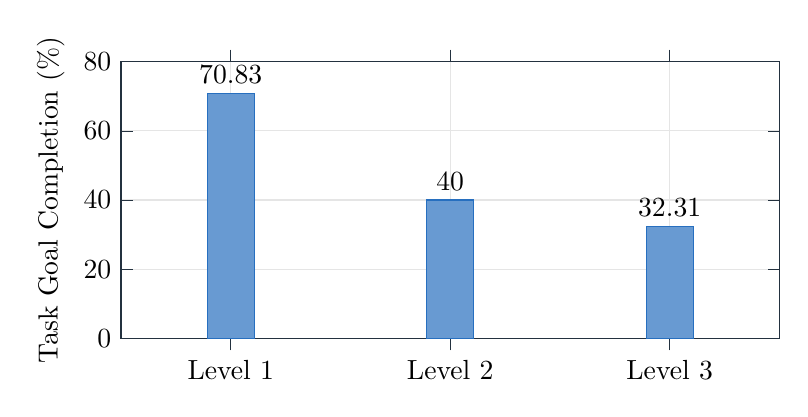
\begin{tikzpicture}
\begin{axis}[
  width=0.82\linewidth,
  height=5.1cm,
  ybar,
  ymin=0,ymax=80,
  ylabel={Task Goal Completion (\%)},
  symbolic x coords={Level 1,Level 2,Level 3},
  xtick=data,
  nodes near coords,
  nodes near coords align={vertical},
  bar width=17pt,
  axis line style={draw=safedark},
  tick style={draw=safedark},
  enlarge x limits=0.25,
  grid=major,
  grid style={draw=black!10}
]
\addplot[fill=safeblue!70,draw=safeblue] coordinates {
  (Level 1,70.83) (Level 2,40.00) (Level 3,32.31)
};
\end{axis}
\end{tikzpicture}
\caption{Measured TGC by AppWorld difficulty. Difficulty comes from the official
task metadata rather than the task identifier.}
\label{fig:difficulty}
\end{figure}

\subsection{Reliability indicators}

\begin{table}[t]
\centering
\caption{Reliability indicators for the AppWorld baseline.}
\label{tab:reliability}
\small
\begin{tabularx}{\linewidth}{@{}YrrY@{}}
\toprule
Indicator & Numerator / denominator & Rate & Interpretation \\
\midrule
No completion call & 90 / 417 & 21.58\% & All 90 tasks failed \\
Reached max turns & 91 / 417 & 21.82\% & Only one task passed \\
False-completion candidates & 153 / 327 & 46.79\% & Completion call followed by evaluator failure \\
Invalid calls & 559 / 15,066 & 3.71\% & Denominator is model-proposed calls \\
Out-of-schema calls & 435 / 15,066 & 2.89\% & All were rejected and not executed \\
Duplicate calls & 987 / 14,631 & 6.75\% & Denominator is executed calls \\
Duplicate writes & 128 / 1,836 & 6.97\% & Observed in 40 tasks \\
\bottomrule
\end{tabularx}
\end{table}

Tasks with an out-of-schema attempt pass at 23.50\% (51/217), compared with
61.50\% (123/200) for tasks without one. Tasks with duplicate calls pass at
15.64\% (28/179), compared with 61.34\% (146/238) without duplicates. Max-turn
tasks pass at 1.10\% (1/91), compared with 53.07\% (173/326) otherwise. These are
descriptive associations, not causal effects; task difficulty and trajectory
length may confound them.

\begin{figure}[t]
\centering
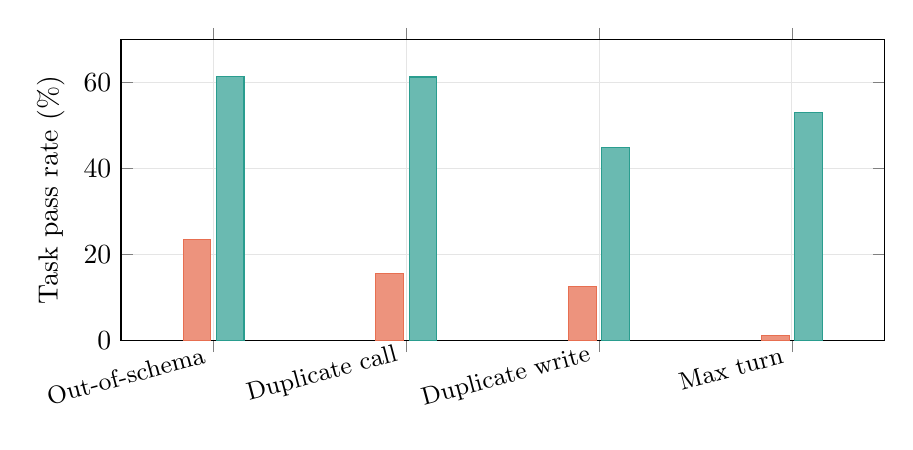
\begin{tikzpicture}
\begin{axis}[
  width=0.93\linewidth,
  height=5.4cm,
  ybar=2pt,
  ymin=0,ymax=70,
  ylabel={Task pass rate (\%)},
  symbolic x coords={Out-of-schema,Duplicate call,Duplicate write,Max turn},
  xtick=data,
  x tick label style={rotate=15,anchor=east,font=\small},
  bar width=10pt,
  grid=major,
  grid style={draw=black!10},
  enlarge x limits=0.16
]
\addplot[fill=safecoral!75,draw=safecoral] coordinates {
  (Out-of-schema,23.50) (Duplicate call,15.64)
  (Duplicate write,12.50) (Max turn,1.10)
};
\addplot[fill=safegreen!70,draw=safegreen] coordinates {
  (Out-of-schema,61.50) (Duplicate call,61.34)
  (Duplicate write,44.83) (Max turn,53.07)
};
\end{axis}
\end{tikzpicture}
\caption{Pass rates conditional on measured trajectory indicators (coral:
present; teal: absent). The plot is associational and must not be interpreted as
an intervention estimate.}
\label{fig:associations}
\end{figure}

\subsection{Failure cost}

\begin{center}
\begin{minipage}{0.70\linewidth}
\centering
\captionof{table}{Efficiency by AppWorld outcome.}
\label{tab:efficiency}
\small
\begin{tabular}{@{}lrrrr@{}}
\toprule
Outcome & Tasks & Mean turns & Mean calls & Mean tokens \\
\midrule
Success & 174 & 9.67 & 18.96 & 130,653 \\
Failure & 243 & 28.46 & 46.63 & 737,614 \\
\bottomrule
\end{tabular}
\end{minipage}
\end{center}

Failed tasks consume 5.65 times as many tokens on average as successful tasks.
The complete run uses 201,973,864 tokens: 195,563,935 input and 6,409,929
output tokens. Reads account for 87.45\% of executed calls. At input/output prices
of CNY 1/2 per million tokens, the estimated cost is CNY 208.38; at CNY 3/6 it
is CNY 625.15. These measurements motivate stagnation and context management but
do not demonstrate that \safedesk{} will realize the projected savings.

\subsection{\texorpdfstring{$\tau^2$}{tau2} diagnostic baseline}

The available $\tau^2$ baseline uses GLM-5 in non-thinking mode as the agent and
DeepSeek V4 Flash in non-thinking mode for the user simulator and judge.

\begin{center}
\begin{minipage}{0.90\linewidth}
\centering
\captionof{table}{Measured 278-task $\tau^2$ diagnostic baseline. DB match is a raw
evaluator component and is not equivalent to final pass, especially in telecom.}
\label{tab:tau2}
\small
\begin{tabular}{@{}lrrrrrr@{}}
\toprule
Domain & Tasks & Pass & DB match & Mean turns & Mean calls & Mean tokens \\
\midrule
Airline & 50 & 64.00\% & 66.00\% & 15.38 & 7.08 & 65,337 \\
Retail & 114 & 79.82\% & 82.46\% & 17.81 & 7.84 & 79,419 \\
Telecom & 114 & 99.12\% & 23.68\% & 37.95 & 6.61 & 253,553 \\
\midrule
Overall & 278 & 84.89\% & 55.40\% & 25.63 & 7.20 & 148,294 \\
\bottomrule
\end{tabular}
\end{minipage}
\end{center}

Across all tasks, the baseline records 25 invalid calls, 11 duplicate non-write
calls, and five recovery attempts, three of which succeed. No confirmed duplicate
write is observed. The 42 failed tasks retain \texttt{unknown}, rather than zero,
for premature finish, partial completion, and unintended side effects. Tokens are
not separated across agent, user simulator, and judge, so the baseline cannot
support a reliable agent-only cost estimate or a matched \safedesk{} comparison.

\subsection{Shadow audit}

Five AppWorld challenge smoke traces were converted to the unified format against
a 457-tool catalog. Conversion produced 129 actions, 129 evidence items, 84
effects, 45 reads, and 84 writes, with no missing tool result or unknown tool. A
conservative shadow audit observed four completion attempts and would block all
four because full task contracts, verified evidence, and verified effects were
unavailable. This demonstrates representational and interception coverage only;
it is not an outcome evaluation and does not establish that each block is correct.

\section{Pending Matched Experiments and Ablations}

\begin{center}
\begin{minipage}{\linewidth}
\centering
\captionof{table}{Frozen main experiment matrix. No pending value is imputed.}
\label{tab:experiments}
\small
\begin{tabularx}{\linewidth}{@{}lYYYrl@{}}
\toprule
ID & Benchmark / split & Model & Runtime & Tasks & Status \\
\midrule
E0 & AppWorld challenge & DeepSeek V4 Flash & Plain function calling & 417 & \measured \\
E1 & AppWorld normal & DeepSeek V4 Flash & Plain function calling & 168 & Rerun pending \\
E2 & AppWorld normal & Qwen3-14B no-thinking & Plain function calling & 168 & \pending \\
E3 & AppWorld challenge & Qwen3-14B no-thinking & Plain function calling & 417 & \pending \\
E4 & AppWorld normal & Qwen3-14B no-thinking & \safedesk & 168 & \pending \\
E5 & AppWorld challenge & Qwen3-14B no-thinking & \safedesk & 417 & \pending \\
E6 & $\tau^2$ three domains & Mixed roles & DeerFlow baseline & 278 & Diagnostic \\
E7/E8 & $\tau^2$ frozen subset & Qwen3-14B no-thinking & Baseline / \safedesk & TBD & \pending \\
\bottomrule
\end{tabularx}
\end{minipage}
\end{center}

\begin{center}
\begin{minipage}{\linewidth}
\centering
\captionof{table}{Planned module ablations. Outcome cells remain empty until execution.}
\label{tab:ablations}
\small
\begin{tabularx}{\linewidth}{@{}lYYcc@{}}
\toprule
ID & Condition & Purpose & TGC & Mean tokens \\
\midrule
A0 & Baseline & Ungoverned control & \pending & \pending \\
A1 & + State \& Verification & Evidence-grounded completion & \pending & \pending \\
A2 & + Tool Execution Guard & Schema, effect, and dependency control & \pending & \pending \\
A3 & + Recovery Controller & Typed recovery and stagnation & \pending & \pending \\
A4 & + Context Manager & Full \safedesk{} runtime & \pending & \pending \\
B1--B4 & Full minus one module & Leave-one-module-out necessity & \pending & \pending \\
\bottomrule
\end{tabularx}
\end{minipage}
\end{center}

The AppWorld leaderboard records Alibaba Cloud ApsaraLab AgentRL with Qwen3-14B
at 86.9\%/80.4\% TGC/SGC on \texttt{test\_normal} and 67.6\%/50.4\% on
\texttt{test\_challenge} \citep{appworldleaderboard2026}. It is an external
reference under different training and execution conditions, not a directly
comparable control. The purpose of E2--E5 is to quantify how much of the gap a
matched runtime intervention can close without weight updates.

\section{Discussion}

\paragraph{Why runtime governance?}
Model capability constrains the quality of plans and action proposals, but real
systems also require deterministic controls. Authentication, amount limits,
idempotency, confirmation, and completion evidence should not depend entirely on
stochastic generation. A structured runtime makes these properties reusable
across models and harnesses.

\paragraph{Accuracy versus conservatism.}
An overly strict completion gate can block a completed task whose evidence was not
captured, while excessive readback adds tokens and latency. Evaluation must
therefore report false blocks, verification coverage, governance overhead, TGC,
and SGC together. Shadow mode should precede enforcement.

\paragraph{Dynamic schema boundaries.}
Out-of-schema calls are a major difficulty marker, but unrestricted schema
expansion increases token cost, ambiguity, and attack surface. Tool resolution
must be scoped to the active subgoal and justified by trace evidence.

\paragraph{Relationship to agentic RL.}
RL can teach better long-horizon action policies; \safedesk{} provides external
state, execution constraints, and auditable recovery. The two may be
complementary. Governed traces may also provide more precise training signals for
future work.

\section{Limitations and Threats to Validity}

\begin{enumerate}[leftmargin=*,itemsep=2pt]
  \item \textbf{The main intervention is unmeasured.} This draft cannot claim
        higher completion, lower cost, or superiority to RL.
  \item \textbf{Historical normal results are invalid for primary claims.} The
        168-task DeepSeek run predates the state-persistence repair; a five-task
        persistence smoke test is not a substitute for a full rerun.
  \item \textbf{The Qwen pilot is not a target baseline.} The existing five-task
        train pilot enabled thinking and is non-representative.
  \item \textbf{Harness differences limit leaderboard comparison.} AppWorld was
        introduced for interactive coding, while our runner uses function calling.
  \item \textbf{Provider versions may drift.} Each run must preserve returned
        model/version metadata, time, parameters, and configuration hashes.
  \item \textbf{Associations are not causal.} Difficulty and trajectory length
        confound out-of-schema, duplicate-call, and max-turn indicators.
  \item \textbf{Some reliability labels require adjudication.} Failed tasks do
        not imply partial completion, premature finish, or side effects.
  \item \textbf{$\tau^2$ tokens are role-mixed.} Formal experiments must separate
        agent, user, and judge usage.
  \item \textbf{Platform faults have affected prior runs.} Persistence, time
        freezing, and Windows GBK encoding require continuous infrastructure checks.
  \item \textbf{Final integration tests are pending.} Code and schema counts do
        not establish implementation correctness.
\end{enumerate}

\section{Ethics and Safety}

\safedesk{} is intended to reduce erroneous side effects, not to expand agent
privilege. The runtime follows least privilege, explicit confirmation, sensitive
field redaction, and traceability. Dynamic tool resolution must not bypass policy;
recovery must not route around permission failures. Released traces and ancillary
data must exclude API keys, account data, personal information, and replayable
credentials. Benchmark writes occur in isolated environments. Real deployment
requires policy review, human takeover, rate and amount limits, rollback, and
incident response.

\section{Conclusion}

\safedesk{} reframes long-horizon tool execution from an unconstrained message
loop into an evidence-grounded state-transition system. Its four modules govern
state and verification, tool execution, typed recovery, and context budgets, while
structured traces support audit and ablation. A complete AppWorld challenge
baseline identifies concrete and measurable failure modes: weak completion
evidence, missing schemas, duplicate actions, stagnation, and extreme token tails.

The system design, core implementation, data protocol, and diagnostic baseline are
complete. The matched Qwen3-14B interventions and ablations remain the necessary
next step. Only after E2--E5 and the module ablations are executed should
\safedesk{} performance claims enter the abstract or conclusion.

\section*{Data Availability}

The accompanying ancillary package contains de-identified task-level derived
tables for 417 AppWorld tasks and 278 $\tau^2$ tasks, aggregate metrics,
experiment and ablation matrices, a metric dictionary, an evidence-claim registry,
source and output SHA-256 manifests, and the deterministic data-construction and
validation scripts. Raw benchmark environments and model traces remain subject to
their original licenses and privacy review.

\appendix
\section{Artifact Validity Register}

\begin{table}[htbp]
\centering
\caption{Validity labels applied before manuscript construction.}
\label{tab:validity}
\small
\begin{tabularx}{\linewidth}{@{}p{0.28\linewidth}p{0.20\linewidth}Y@{}}
\toprule
Artifact & Validity & Reason \\
\midrule
DeepSeek challenge, 417 tasks & Primary measured & Persistence repaired;
UTF-8 failures rerun; final states reevaluated \\
DeepSeek normal, 168 tasks & Invalid for primary claim & Predates persistence correction \\
Persistence check, 5 tasks & Smoke only & Selected sample is non-representative \\
Qwen3-14B train, 5 tasks & Invalid for target baseline & Thinking enabled; train pilot \\
State/verification shadow, 5 traces & Diagnostic only & Contracts and verified evidence incomplete \\
Trace conversion, 5 traces & Implementation diagnostic & Coverage, not effectiveness \\
\bottomrule
\end{tabularx}
\end{table}

\section{Metric Definitions}

\begin{table}[htbp]
\centering
\caption{Core metric definitions and denominators.}
\label{tab:metrics}
\small
\begin{tabularx}{\linewidth}{@{}p{0.25\linewidth}YY@{}}
\toprule
Metric & Definition & Unit / denominator \\
\midrule
TGC & Successful tasks divided by valid tasks & Task \\
SGC & Scenarios for which all variants pass divided by complete scenarios & Scenario \\
False-completion rate & Confirmed unsupported completion claims divided by completion attempts & Task \\
Max-turn rate & Tasks reaching the configured cap divided by valid tasks & Task \\
Invalid-call rate & Invalid proposed calls divided by all model-proposed calls & Call \\
Out-of-schema rate & Calls absent from the active schema divided by proposed calls & Call \\
Duplicate-write rate & Duplicate write actions divided by executed writes & Write call \\
Verification coverage & Verified required effects divided by required effects & Effect \\
Recovery success & Successful recoveries divided by triggered recoveries & Recovery \\
Token statistics & Mean, median, P95, and maximum reported usage & Task \\
\bottomrule
\end{tabularx}
\end{table}

\section{Reproducibility Checklist}

\begin{itemize}[leftmargin=*,itemsep=1pt]
  \item Unique run ID: experiment, task, trial, and configuration hash.
  \item Atomic per-task result writes and schema-validated aggregation.
  \item Model, predictor, simulator, judge, and evaluator roles recorded separately.
  \item Final-state persistence asserted before evaluation.
  \item Infrastructure failures classified and rerun under the identical condition.
  \item Code commit, task-list hash, model version, request parameters, and source
        hashes preserved with each aggregate.
  \item Pending claims remain blocked in the claim registry until matched evidence
        is available.
\end{itemize}

\bibliographystyle{plainnat}
\bibliography{references}

\end{document}
